\section{Failure cases of \textsc{sqair}}
\label{app:fail}

\begin{center}
    \centering
    \begin{minipage}[c]{0.65\linewidth}
        \centering
        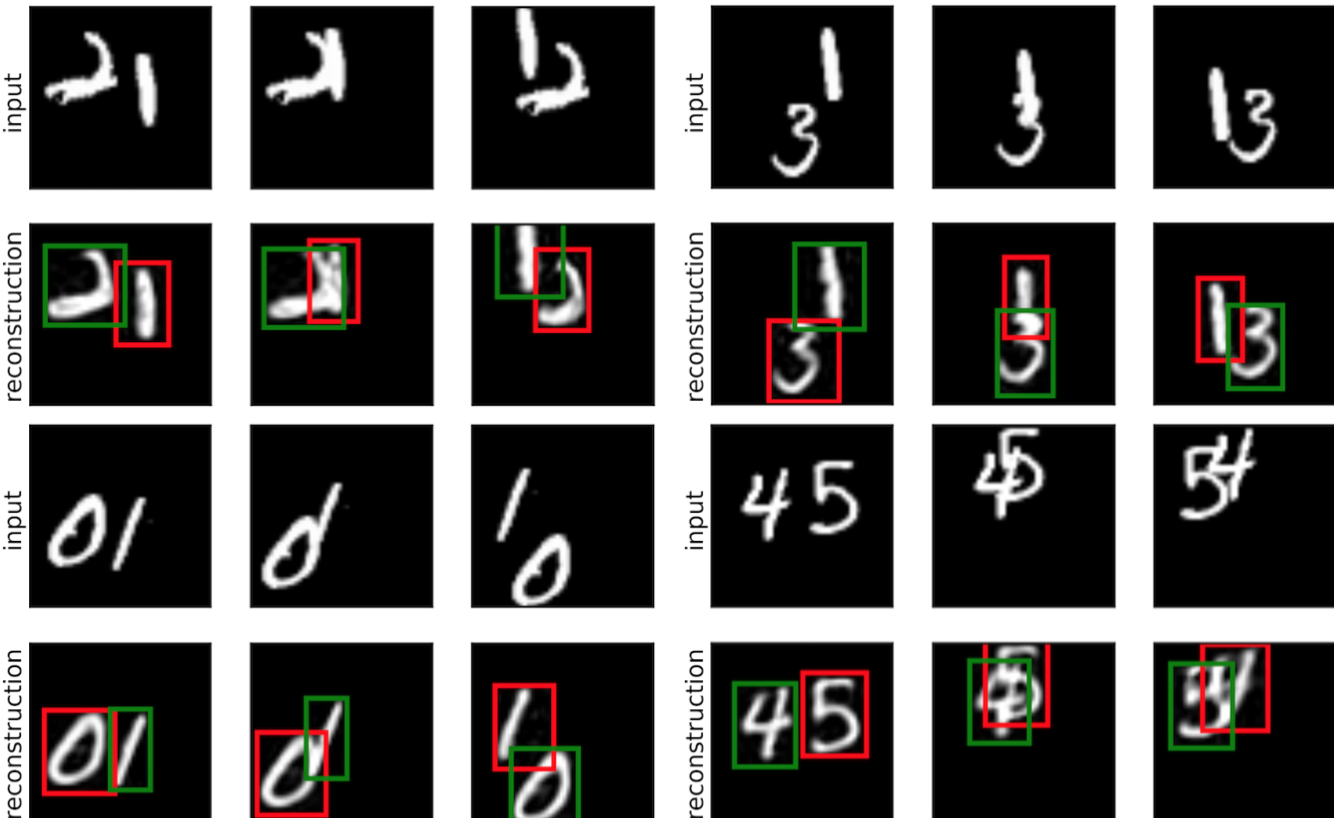
\includegraphics[width=\linewidth]{figures/SQAIR/sqair_id_swap}
    \end{minipage}
    \hfill
    \begin{minipage}[c]{0.33\linewidth}
    \centering
        \captionof{figure}{Examples of ID swaps in a version of \gls{SQAIR} \textit{without} proposal glimpse extraction in \gls{prop} (see \Cref{app:algo} for details). Bounding box colours correspond to object index (or its identity). When \gls{prop} is allowed the same access to the image as \gls{disc}, then it often prefers to ignore latent variables, which leads to swapped inference order.}
        \label{fig:id_swap}
    \end{minipage}
\end{center}
\begin{center}
    \centering
    \begin{minipage}[c]{0.65\linewidth}
        \centering
        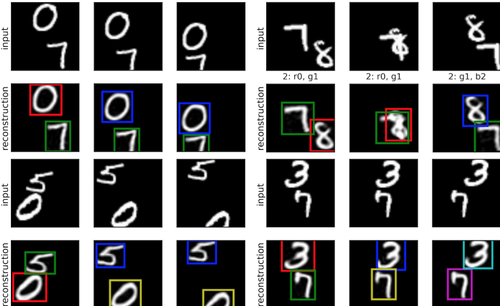
\includegraphics[width=\linewidth]{figures/SQAIR/sqair_redetect}
    \end{minipage}
    \hfill
    \begin{minipage}[c]{0.33\linewidth}
        \centering
        \vspace{8pt}
        \captionof{figure}{Examples of re-detections in \textsc{mlp}-\gls{SQAIR}. Bounding box colours correspond to object identity, assigned to it upon discovery. In some training runs, \gls{SQAIR} converges to a solution, where objects are re-detected in the second frame, and \gls{prop} starts tracking only in the third frame (left). Occasionally, an object can be re-detected after it has severely overlapped with another one (top right). Sometimes the model decides to use only \gls{disc} and repeatedly discovers all objects (bottom right). These failure mode seem to be mutually exclusive -- they come from different training runs.}
        \label{fig:redetect}
    \end{minipage}
\end{center}

\begin{center}
    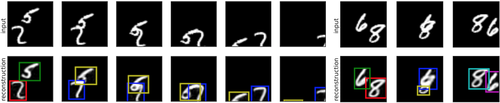
\includegraphics[width=\linewidth]{figures/SQAIR/sqair_weird_rec}
    \captionof{figure}{Two failed reconstructions of \gls{SQAIR}.
        \textit{Left}:
            \Gls{SQAIR} re-detects objects in the second time-step. Instead of 5 and 2, however, it reconstructs them as 6 and 7. Interestingly, reconstructions are consistent through the rest of the sequence.
        \textit{Right:}
            At the second time-step, overlapping 6 and 8 are explained as 6 and a small 0. The model realizes its mistake in the third time-step, re-detects both digits and reconstructs them properly.
    }
    \label{fig:weird_rec}
\end{center}